
\documentclass[12pt]{article}
\usepackage[utf8]{inputenc}

\usepackage[a4paper, margin=1in]{geometry}

\usepackage{newtxtext}
\usepackage{amsmath,amssymb,amsthm}
\usepackage{newtxmath} % must come after amsXXX

\usepackage{float}%防止图片乱跑



\usepackage{graphicx}
%\usepackage{subfigure}




\usepackage{xcolor}
\usepackage{fancyhdr}

\usepackage{listings}
%\usepackage{ctex}

\usepackage{booktabs}


%%%%%%%%%%%% for sudocode %%%%%%%
\usepackage{algorithm}
\usepackage{algpseudocode}
%%%%%%%%%%%%%%%%%%%%%%%%%%%%%%%%%




%%%%%%%%%%%%%%%%%%%%%%%%%%%%%%%%%%%%%%%%%%%%%%%%%%%%%%%%%%%%%%%
%%%%%%%%%%%%%%%%%%%%%%%%%%%%%%%%%%%%%%%%%%%%%%%%%%%%%%%%%%%%%%%

\begin{document}

\title{530.767 CFD\\Spring 2024\\HW 2–Haobo Zhao}
\maketitle

For this project, we use different schemes to solve
1D Burger's equation numerically: For Forwar in Time Central
in Space (FTCS) and Quadratic UPwind Interpolation Convection
Kinematic (QUICK) schemes, we found it do have potential 
oscillation problem, which could be showned also in modified 
equation's diffusion term's subtracted time difference term. 
For UPwind scheme, we found it have added viscosity problem,
which could also be shown in modified equation's dissipation
term, where its viscosity been added by spacial difference term.

\tableofcontents


\section{Question Review}

1) Consider the viscous Burger's equation:
\begin{equation}
    u_t + u_x = \frac{1}{\text{Pe}} u_{xx} ; \quad 0 
    \leq x \leq 1
\end{equation}
where Pe=50, with \( u(0,t) = 0 \), \( u(1,t) = 1 \) and 
\( u(x,0) = 0 \).\\

Solve the above problem using FTCS scheme. Use grids with 
spacing of 1/20, 1/50 and 1/100. For all these grids, choose 
a single time-step size that provides stable solution for the 
finest grid. Demonstrate that oscillatory solutions are 
obtained for \( \text{Pe}\Delta x > 2 \), while the solutions 
are smooth for \( \text{Pe}\Delta x < 2 \).\\




\noindent 2) Repeat the above problem with a
\begin{enumerate}
    \item[a.] 1\textsuperscript{st}-upwind scheme, and
    \item[b.] 2\textsuperscript{nd} order upwind scheme for the convection term.
    \item[c.] QUICK Scheme
\end{enumerate}
Compare the results for all the cases against the exact 
solution and comment on the behavior of the solution.
What effective viscosity do you see for the various upwind 
cases, and does it correspond well to what you expect from 
the modified equation for the various schemes?


\section{1.FTCS Scheme analysis with $Pe\Delta x$}
\subsection{FTCS Scheme}

For the FTCS scheme, which is means Forward difference in Time,
Cnetral difference in Space. 

\subsubsection{FTCS Iteration Formula}

For general Burger's Equation:
$$
u_t + cu_x = {\nu} u_{xx}
$$

Discrete this PDE using forward difference in time,
central difference in space (FTCS), we could get:

$$
\frac{u_i^{n+1} - u_i^n}{\Delta t} + c \frac{u_{i+1}^n - u_{i-1}^n}{2\Delta x} = \nu \frac{u_{i+1}^n - 2u_i^n + u_{i-1}^n}{\Delta x^2} \\
$$\\

Organize this equation, we could obtain:

$$
u_i^{n+1} = (\frac{\nu \Delta t}{(\Delta x)^2} - \frac{c\Delta t}{2\Delta x})u_{i+1}^n + (1-2r)u_i^n + (\frac{\nu \Delta t}{(\Delta x)^2}  + \frac{c\Delta t}{2\Delta x})u_{i-1}^n \\
$$\\

As \( r = \frac{\nu \Delta t}{\Delta x^2} \), \( C = \frac{\Delta t}{2\Delta x} \),
we could obtain:

$$
u_i^{n+1} = (r - \frac{C}{2})u_{i+1}^n + (1-2r)u_i^n +  (r + \frac{C}{2})u_{i-1}^n
$$\\

As our Equation is \( u_t + u_x = \frac{1}{\text{Pe}} u_{xx} \), 
we can find \( c = 1 \),
$\nu = \frac{1}{Pe}$,
could get 
 $$ r = \frac{\Delta t}{\text{Pe}\Delta x^2} , C = \frac{\Delta t}{\Delta x} $$

Then, the iteration formula for FTCS scheme is:

$$
u_i^{n+1} = r(1 - \frac{\text{Pe}\Delta x}{2})u_{i+1}^n + (1-2r)u_i^n + r (1 + \frac{\text{Pe}\Delta x}{2})u_{i-1}^n
$$



To full fill the stability requirement:

$$
2C =< Pe\Delta x =<\frac{2}{C}
$$

Where we choose  $\Delta t =0.0001$
\subsubsection{Solver architecture}

\begin{figure}[H]
    \centering
    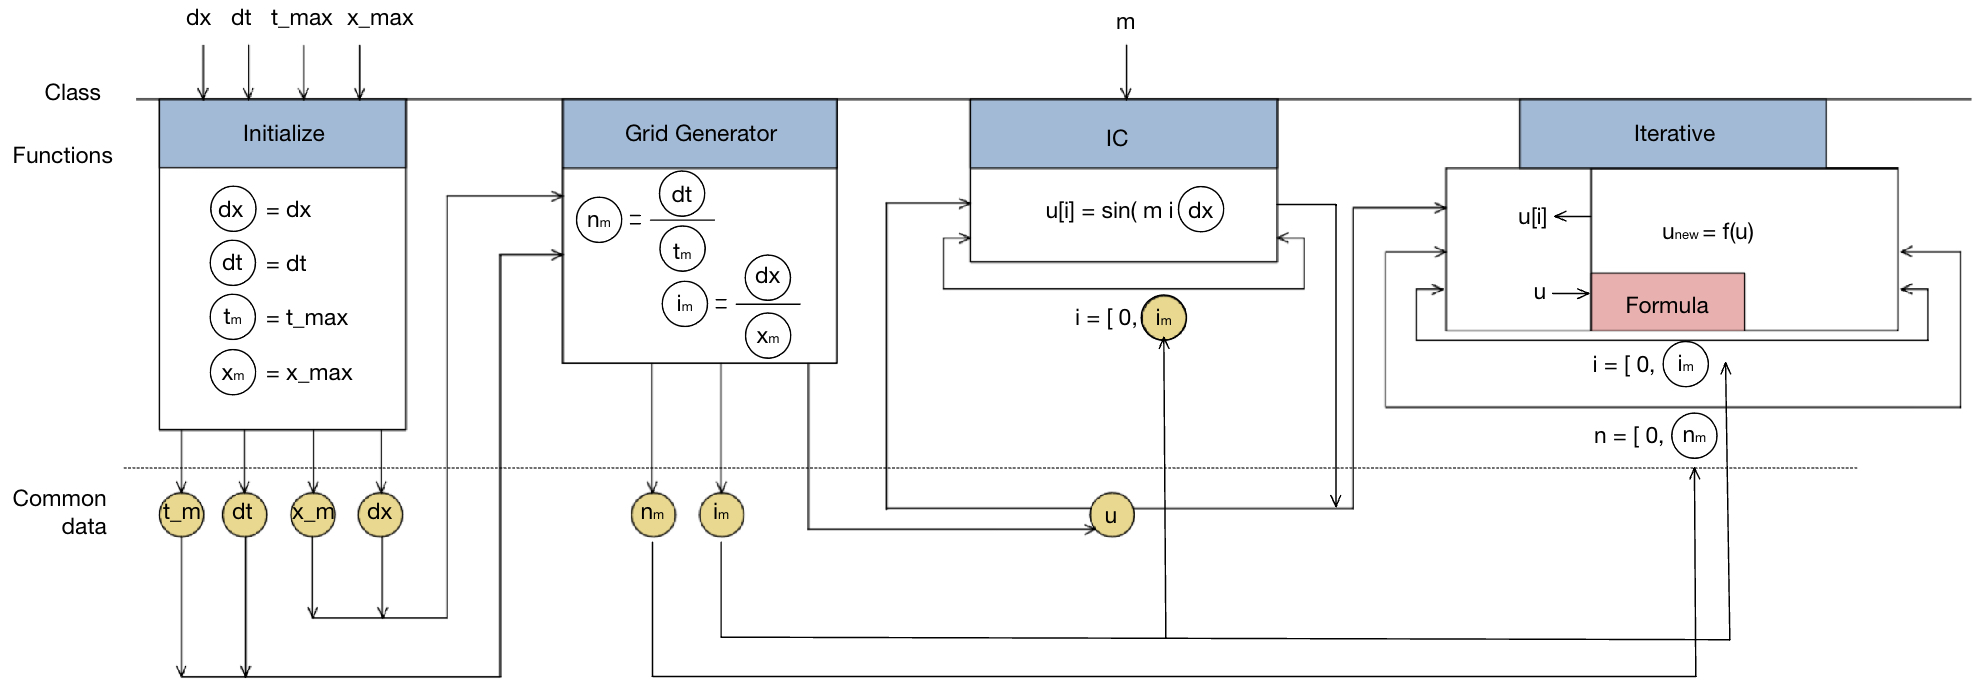
\includegraphics[width=1\textwidth]{figures/Solver_architecture.jpg}
    \label{IGs.jpg}
    \caption{Solver Architecture}
\end{figure}

The solver architecture is showing above. As we put our iteration
formula for one point iteration, other schemes are also using 
same solver but with the replaced iteration formula.




\subsection{Exact solution}

The exact solution of this problem is:


$$
u(\infty,x) = \frac{e^{xPe}-1}{e^{Pe}-1}
$$





\subsection{FTCS Scheme Result}
Iteration until its reaches steady state,
the result is showing below:


\begin{figure}[H]
    \centering
    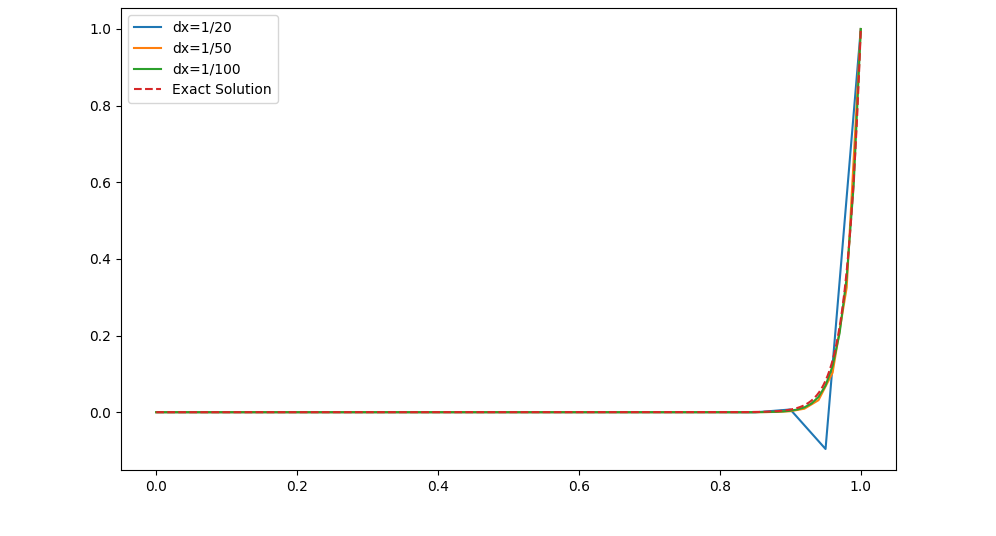
\includegraphics[width=0.8\textwidth]{figures/P1t0.1All.png}
    \label{IGs.jpg}
    \caption{FTCS with different dx}
\end{figure}


By ploting results in different dx in same figure, we could
find for dx=1/50, and dx=1/100, it is pretty close to the exact
solution. For dx=1/20, we could see there is negative point, 
where the oscillation occur.\\



For more detailed comparsion around 1 (which is also the 
changeing part), the result is showing below:




\begin{figure}[H]
    \centering
    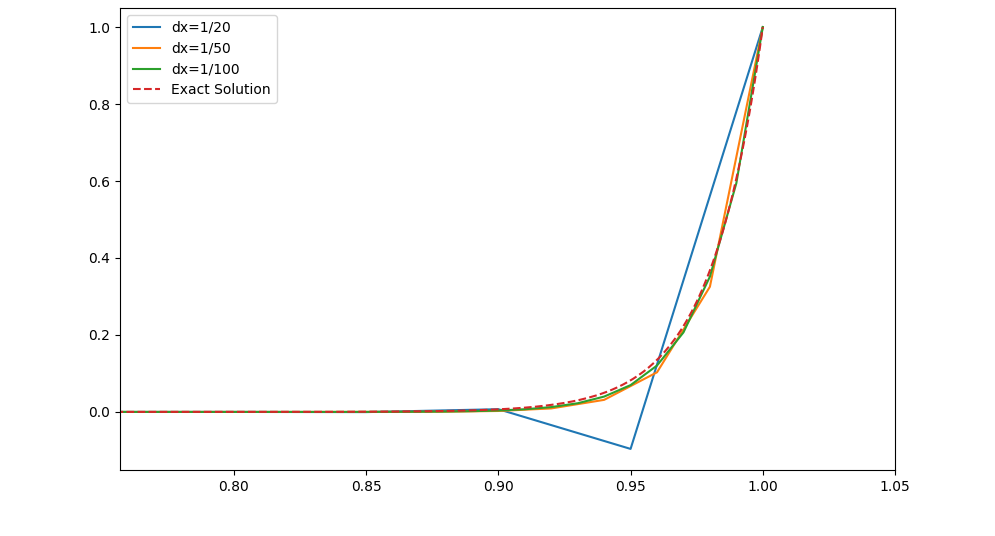
\includegraphics[width=0.8\textwidth]{figures/P1t0.1AllH.png}
    \label{IGs.jpg}
    \caption{FTCS with different dx (detailed)}
\end{figure}


\subsection{Result analysis}
As the problem suuggested, we are using $Pe\Delta x$ to divide
our result group:

$$
Pe \Delta x = \frac{C}{r} = \frac{c \Delta x}{\nu} = Pe \cdot \Delta x = 50 \Delta x
$$

When we let $Pe\Delta x$>2, where is dx>2/50, qualify for the 
scheme dx=1/20, could see some oscillation. Mean while, the
other scheme dx<2/50, which is dx=1/50 and dx=1/100,
do not have such oscillation, full fill our expectation.




\section{2.Different scheme analysis with Modified Equation}

For this section, we compared different schemes in convection 
term: Central difference (See detail in pervious section), 
1st order UPwind scheme, 2nd order UPwind scheme, and QUICK
scheme.

\subsection{Iteration Formula for UPwind schemes and QUICK 
scheme}

\subsubsection{1st UPwind scheme iteration formula}

For general Burger's Equation:
$$
u_t + cu_x = {\nu} u_{xx}
$$

Discrete this PDE using forward difference in time,
1st UPwind for convergence term, we could get:

$$
\frac{u_i^{n+1} - u_i^n}{\Delta t} + c \frac{u_{i}^n - u_{i-1}^n}{\Delta x} = \nu \frac{u_{i+1}^n - 2u_i^n + u_{i-1}^n}{\Delta x^2} \\
$$\\

Organize this equation, we could obtain:

$$
u_i^{n+1} = (\frac{\nu \Delta t}{(\Delta x)^2})u_{i+1}^n + (1-2r+\frac{c\Delta t}{\Delta x})u_i^n + (\frac{\nu \Delta t}{(\Delta x)^2}  + \frac{c\Delta t}{\Delta x})u_{i-1}^n \\
$$\\

As \( r = \frac{\nu \Delta t}{\Delta x^2} \), \( C = \frac{\Delta t}{2\Delta x} \),
we could obtain the iteration formula for 1st UPwind scheme:

$$
u_i^{n+1} = r u_{i+1}^n + (1-2r +C)u_i^n +  (r + C)u_{i-1}^n
$$\\

As our Equation is \( u_t + u_x = \frac{1}{\text{Pe}} u_{xx} \), 
we can find \( c = 1 \),
$\nu = \frac{1}{Pe}$,
could get 
 $$ r = \frac{\Delta t}{\text{Pe}\Delta x^2} ,  C = \frac{\Delta t}{\Delta x} $$



\subsubsection{2nd UPwind scheme iteration formula}
The BUrger equation is:
\[
u_t + c u_x = \nu u_{xx}
\]

For 2nd UPwind scheme for convection term, it could been shown
as:

\[
\frac{\Delta u_i}{\Delta t} + c \frac{\nabla_{2x} u_i}{2 \Delta x} - \nu \frac{\delta^2_{xx} u_i}{\Delta x^2}
\]

Where
$$
\begin{cases}
\Delta u_i = u_i^{n+1} - u_i^{n} &\\

\nabla_{2x} u_i = 3 u_i - 4 u_{i+1} + u_{i-2} &\\

\delta^2_{xx} u_i = u_{i+1} - 2 u_i + u_{i-1} &
\end{cases}
$$


Could get the iteration formula:

\[
u_{i+1} = u_i - \frac{c \Delta t}{2 \Delta x} \nabla_x u_i + \frac{\nu \Delta t}{\Delta x^2} \delta^2_x u_i
\]

As our Equation is \( u_t + u_x = \frac{1}{\text{Pe}} u_{xx} \), 
we can find \( c = 1 \),
$\nu = \frac{1}{Pe}$,
could get 
 $$ r = \frac{\Delta t}{\text{Pe}\Delta x^2} ,  C = \frac{\Delta t}{\Delta x} $$

Where our iteration formula could be shown as:
\[
u_{i+1} = u_i - \frac{C}{2} \nabla_{2x} u_i + r \delta^2_{xx} u_i
\]

Where
$$
\begin{cases}
\nabla_{2x} u_i = 3 u_i - 4 u_{i+1} + u_{i-2} &\\
\delta^2_{xx} u_i = u_{i+1} - 2 u_i + u_{i-1} &
\end{cases}
$$


\subsubsection{QUICK Scheme iteration formula}
Quadratic UPwind Interpolation for Convection Kinematic (QUICK)
could be shown below:

\[
u_{i+1} = u_i - \frac{C}{2} Q_x(u_i) + r \delta^2_{xx} u_i
\]


Where

\[
    Q_x(u_i)={U_e - U_w} = \left( \frac{1}{8} U_p + \frac{3}{8} U_e - \frac{1}{8} U_w \right) - \left( \frac{1}{8} U_w + \frac{3}{8} U_p - \frac{1}{8} U_m \right)
\]

                                                                                        

\subsection{Result and compare}

\subsubsection{1st UPwind scheme result}
\begin{figure}[H]
    \centering
    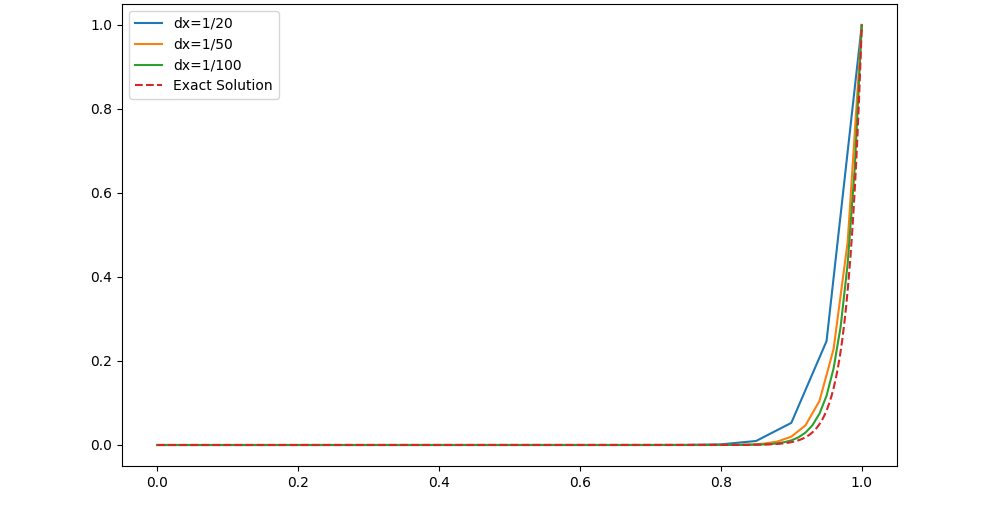
\includegraphics[width=0.8\textwidth]{figures/P2U1t0.1.png}
    \label{IGs.jpg}
    \caption{1st UPwind scheme result }
\end{figure}

For the 1st UPwind scheme, could find whatever the dx is,
the FDE result's divergence is much higher than the exact 
solution. 

\subsubsection{2nd UPwind scheme result}

\begin{figure}[H]
    \centering
    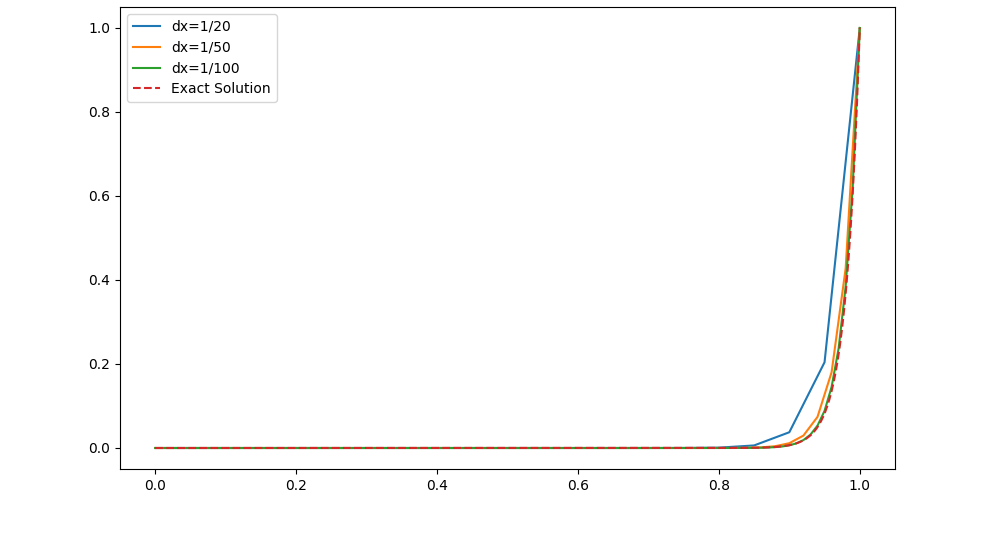
\includegraphics[width=0.8\textwidth]{figures/P2U2t0.1.png}
    \label{IGs.jpg}
    \caption{2nd UPwind scheme result}
\end{figure}

Same result for 2nd UPwind scheme, the high viscosity 
could been easily observed. It is little better than
1st UPwind though.


\subsubsection{QUICk scheme result}
\begin{figure}[H]
    \centering
    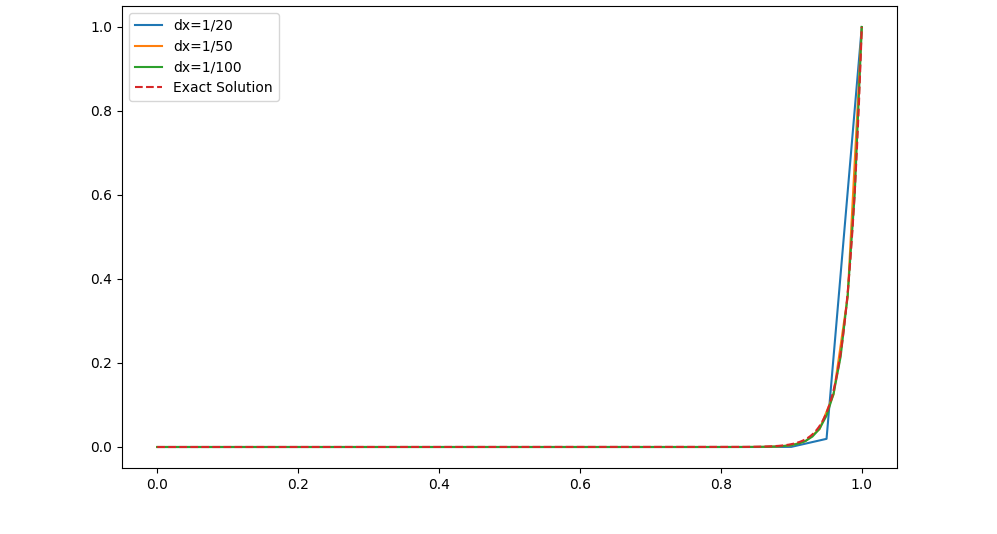
\includegraphics[width=0.8\textwidth]{figures/P2Qt0.1.png}
    \label{IGs.jpg}
    \caption{QUICK scheme result}
\end{figure}

For the quick scheme, we could say it is much better, and 
does not show abnormal divergence (viscosity), which result 
is pretty close to the exact solution. The more detailed 
result is showing below:



\begin{figure}[H]
    \centering
    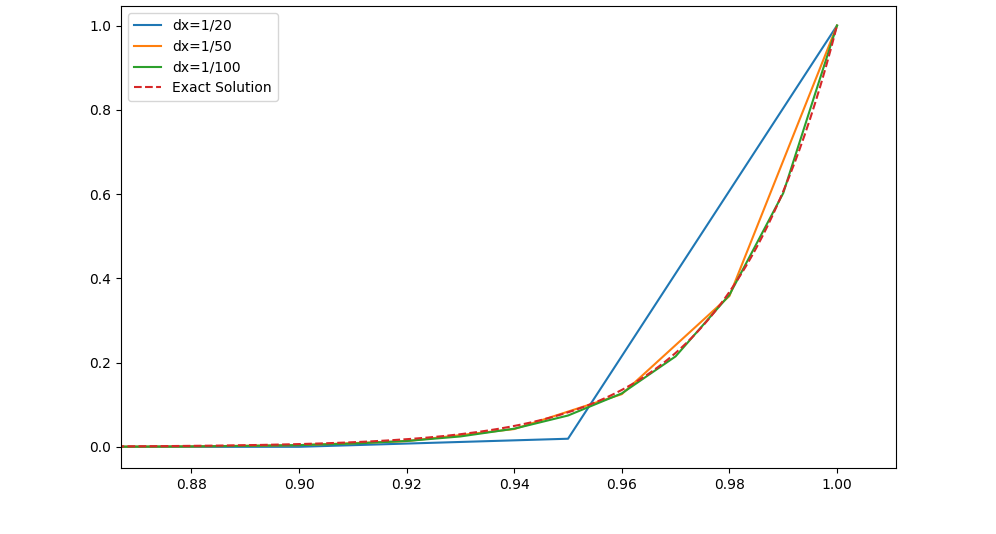
\includegraphics[width=0.8\textwidth]{figures/P2Qt0.1H.png}
    \label{IGs.jpg}
    \caption{QUICK scheme result (detailed)}
\end{figure}





\subsection{Result analysis}

\subsubsection{Modified Wavenumber}


We could get the modified equations (Steps please see Appendix):

FTCS:
\[ u_t + c u_x = \left( \nu - \frac{c^2 \Delta t}{2} \right) u_{xx} \]

1st Upwind scheme:
\[ u_t + c u_x = \left( \nu - \frac{1}{2} \Delta t c^2 + \frac{1}{2} (c \Delta x) \right) u_{xx} \]

QUICK:
\[ u_t + c u_x = \left( \nu - \frac{c^2 \Delta t}{2} \right) u_{xx} \]

These modified equation are derived as ignore high order 
$\Delta$ and derivative higher than 2nd order.


\subsubsection{Result analysis with modified equation}

From the result of UPwind schemes, we could found that their
numerical solution is little bit ``increased'' at the diffusion
close to the right boundary (source), which is due to 
the added viscosity in the modified equation. For QUICK scheme,
its modified equation do not have such added viscosity term,
which its result is pretty close to the exact solution.\\

For more analysis based on the modified equation, we could
find in FTCS and QUICK, the modified equation's dissipation
term is actually been subtracted by term with $\Delta t$, 
which make the dissipation term could be negative (with some
$\Delta x$ and $\Delta t$), which could cause oscillation.

FTCS:
\[ u_t + c u_x = \left( \nu - \frac{c^2 \Delta t}{2} \right) u_{xx} \]


QUICK:
\[ u_t + c u_x = \left( \nu - \frac{c^2 \Delta t}{2} \right) u_{xx} \]




Could seen, for FTUS, $\Delta x =1/20$ could show oscillation,
for QUICK, $\Delta x =1/10$, could also show oscillation:

\begin{figure}[H]
    \centering
    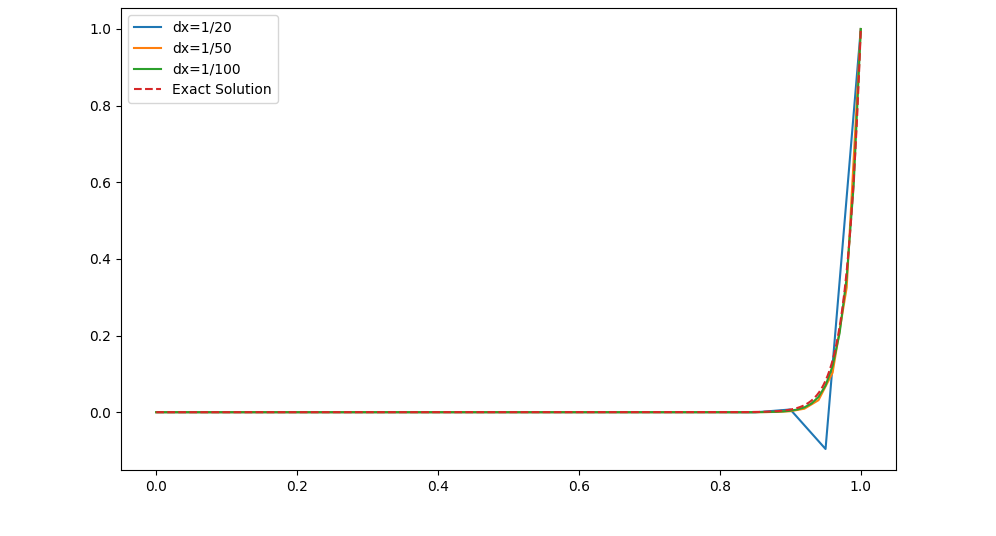
\includegraphics[width=0.49\textwidth]{figures/P1t0.1All.png}
    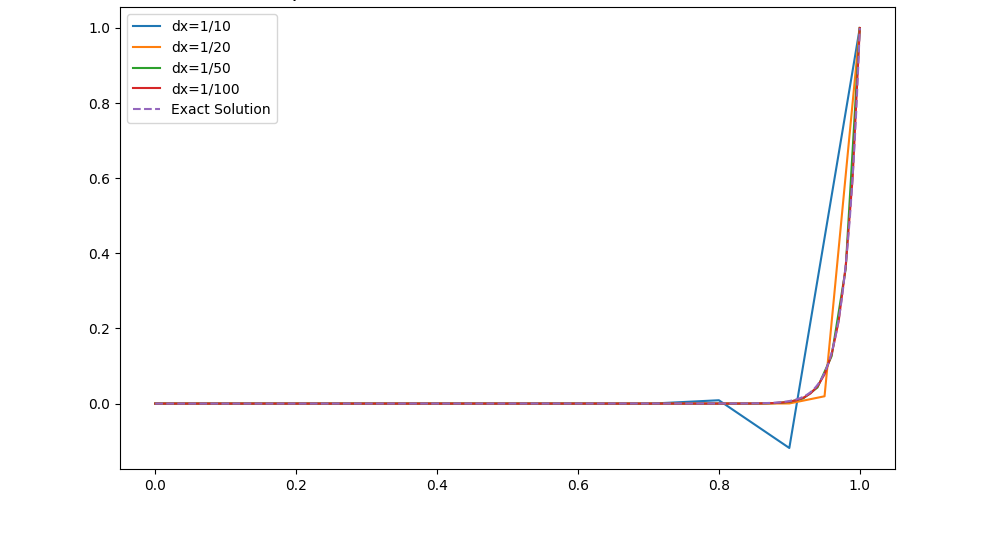
\includegraphics[width=0.49\textwidth]{figures/P2Qosc.png}
    \label{IGs.jpg}
    \caption{FTUS and QUICK oscillation}
\end{figure}



For UPwind scheme, we could find its viscosity been subtract 
term with $\Delta t$ same time added term of $\Delta x$, which
could make our equation cancel the oscillation, but could
cause viscosity abnormally added up, showing on the result:


\begin{figure}[H]
    \centering
    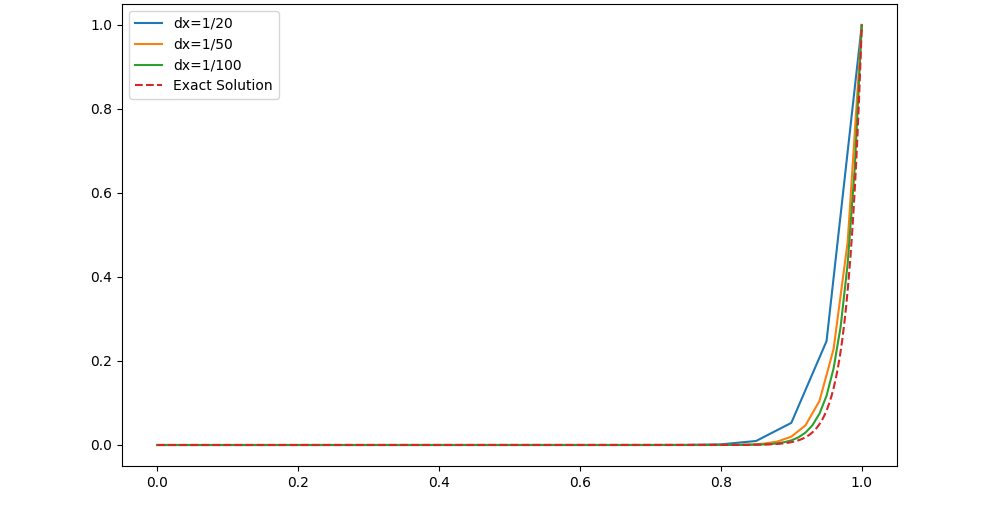
\includegraphics[width=0.8\textwidth]{figures/P2U1t0.1.png}
    \label{IGs.jpg}
    \caption{1st UPwind scheme result }
\end{figure}


1st Upwind scheme:
\[ u_t + c u_x = \left( \nu - \frac{1}{2} \Delta t c^2 + \frac{1}{2} (c \Delta x) \right) u_{xx} \]

We could find the dissipation term has one addition and one 
subtraction, which let us to think:
if there is a possibility to make the dissipation term exactly
the viscosity? 

\subsubsection{Possibility to get exact viscosity}

Let the viscosity exactly back to normal, we just need 
to let:
$$
\frac{1}{2} \Delta t c^2 = \frac{1}{2} (c \Delta x)
$$

Where is

$$
c \Delta t = \Delta x
$$

However, it cannot full fill Stability condition.































%%%%%%%%%%%%%%%%%%%%%%%%%%%%%%%%%%%%%%%%%%%%%%%%%%%%%%%%%%%%%%%
%%%%%%%%%%%%%%%%%%%%%%%%%%%%%%%%%%%%%%%%%%%%%%%%%%%%%%%%%%%%%%%
%%%%%%%%%%%%%%%%%%%%%%%%%%%%%%%%%%%%%%%%%%%%%%%%%%%%%%%%%%%%%%%
\newpage
\section*{Appendix}
% 在目录中添加Appendix
\addcontentsline{toc}{section}{Appendix}
\begin{scriptsize}

    \textbf{Modified Equation Steps}

    We could calculate different scheme's truncation error:
    \(\Delta t\) means forward difference in time:
    \begin{align*}
        \Delta_t u_i &= u_i^{n+1} - u_i^n \\
        \Delta_t u_i &= \Delta t u_{i_t} + \frac{1}{2}(\Delta t)^2 u_{i_{tt}} + \frac{1}{3!}(\Delta t)^3 u_{i_{ttt}} + \mathcal{O}((\Delta t)^4)
    \end{align*}
    
    \(\Delta_x\) means forward difference in space (\(x\)):
    \begin{align*}
        \Delta_x u_i &= u_{i+1} - u_i \\
        \Delta_x u_i &= \Delta x u_{i_x} + \frac{1}{2}(\Delta x)^2 u_{i_{xx}} + \frac{1}{3!}(\Delta x)^3 u_{i_{xxx}} + \mathcal{O}((\Delta x)^4)
    \end{align*}
    
    \(\nabla_x\) means backward difference in space (\(x\)):
    \begin{align*}
        \nabla_x u_i &= u_i - u_{i-1} \\
        \nabla_x u_i &= \Delta x u_{i_x} - \frac{1}{2}(\Delta x)^2 u_{i_{xx}} + \frac{1}{3!}(\Delta x)^3 u_{i_{xxx}} + \mathcal{O}((\Delta x)^4)
    \end{align*}
    
    For the second order backward difference:
    \begin{align*}
        \nabla_{2x} u_i &= 2u_i - 4u_{i+1} + u_{i+2} \\
        &= 4(\Delta x u_{i_x} - \frac{1}{2}(\Delta x)^2 u_{i_{xx}} + \frac{1}{3!}(\Delta x)^3 u_{i_{xxx}}) + (-2\Delta x u_{i_x} + 2(\Delta x)^2 u_{i_{xx}} - \frac{4}{3}(\Delta x)^4 u_{i_{xxxx}}) \\
        \nabla_{2x} u_i &= 2 \Delta x u_{i_x} + \frac{2}{3}(\Delta x)^3 u_{i_{xxx}}
    \end{align*}
    
    \(\delta_x\) means central difference in space (\(x\)):
    \begin{align*}
        \delta_x u_i &= u_{i+1} - u_{i-1} \\
        \delta_x u_i &= 2\Delta x u_{i_x} + \frac{1}{3!}(\Delta x)^3 u_{i_{xxx}} + \mathcal{O}((\Delta x)^4)
    \end{align*}
    
    For the second order central difference:
    \begin{align*}
        \delta_x^2 u_i &= u_{i+1} + u_{i-1} - 2u_i; \\
        \delta_x^2 u_i &= (\Delta x)^2 u_{i_{xx}} + \frac{1}{12}(\Delta x)^4 u_{i_{xxxx}} + \ldots
    \end{align*}
    

\begin{lstlisting}[language=python,caption={Problem1, Py code for FTCS Solver}]



    import math

    import numpy as np
    
    import matplotlib.pyplot as plt
    import matplotlib as mpl
    import copy
    
    class FTCS_Solver:
        def __init__(self, dx, dt, x_max, t_max):
            self.dx = dx
            self.dt = dt
            self.x_max = x_max
            self.t_max = t_max
    
        def grid_generate(self):
            self.i_max = int(self.x_max/self.dx)
            self.n_max = int(self.t_max/self.dt)
    
            self.u = np.zeros(( self.i_max +1 ))
    
        def IC(self):
            for i in range(0, self.i_max+1):
                self.u[i] = 0
    
        def Iteration_Formula(self, u_W, u_E, u):
            self.Pe = 50
            Pe = self.Pe
            C = self.dt/self.dx
            r = ((1/Pe)*self.dt)/(self.dx**2)
    
            u_new = (r-C/2)*u_E + (1-2*r)*u + (r+C/2)*u_W
    
            return u_new
    
        def Iterative(self):
            u_Next = copy.deepcopy(self.u)
            
            self.Pe = 50
    
            for n in range(0, self.n_max):
                u_Next[0] = 0
                for i in range(1,self.i_max):
                    u_Next[i] = self.Iteration_Formula(self.u[i-1], self.u[i+1], self.u[i])
                u_Next[self.i_max] = 1
                self.u = u_Next
    
            return self.u
        
        def plot_result(self):
            x = np.arange(0,self.i_max+1)
            plt.plot(x,self.u)
            plt.show()
    
    
    
        
    
    
    def Runner(dx, dt, x_max, t_max):
    
        u_Final = 0
    
        Run = FTCS_Solver(dx, dt, x_max, t_max)
    
        Run.grid_generate()
    
        Run.IC()
    
        u_Final = Run.Iterative()
    
        return u_Final
    
    
    
    def plot_result(x_max, t_max, dx_20, dx_50, dx_100, u_20, u_50, u_100):
        x_20 = np.linspace(0, x_max, len(u_20))
        x_50 = np.linspace(0, x_max, len(u_50))
        x_100 = np.linspace(0, x_max, len(u_100))
    
        x_e = np.linspace(0,1,1000)
        u_e = u_exact(x_e)
    
        plt.figure(figsize=(10, 6))
    
        plt.plot(x_20, u_20, label='dx=1/20')
        plt.plot(x_50, u_50, label='dx=1/50')
        plt.plot(x_100, u_100, label='dx=1/100')
        plt.plot(x_e, u_e, linestyle='--', label='Exact Solution')
    
        plt.legend()
        plt.title('Numerical at t=%f vs. Exact Final Solution '%t_max)
    
    
        plt.show()
    
    
    
    def u_exact(x):
        Pe = 50
        return (np.exp(x*Pe)-1)/(np.exp(Pe)-1)
    
    
    
        
    
    
        
        
    
        
    
    
        
    
    class Post_op(FTCS_Solver): #UNFINISH!!!!! DO NOT FORGRT
        
    
        pass
    
            
    
    
    
    
    
    def main():
    
        x_max = 1
    
        t_max = 1
    
        dx = 1/20
        dt = 0.0001
    
        dx_20 = 1/20
        u_20 = Runner(dx_20, dt, x_max, t_max)
    
        dx_50 = 1/50
        u_50 = Runner(dx_50, dt, x_max, t_max)
    
        dx_100 = 1/100
        u_100 = Runner(dx_100, dt, x_max, t_max)
    
        plot_result(x_max, t_max, dx_20, dx_50, dx_100, u_20, u_50, u_100)
    
    
    
    
    
        
    
    
    
    
    
    
    
    if __name__ == '__main__':
        main()
    
    
    
    
    
    
    
    
    
        


\end{lstlisting}


\begin{lstlisting}[language=python,caption={Problem2, 1st UPwind Solver updated}]


    import math

    import numpy as np
    
    import matplotlib.pyplot as plt
    import matplotlib as mpl
    import copy
    
    class FTCS_Solver:
        def __init__(self, dx, dt, x_max, t_max):
            self.dx = dx
            self.dt = dt
            self.x_max = x_max
            self.t_max = t_max
    
        def grid_generate(self):
            self.i_max = int(self.x_max/self.dx)
            self.n_max = int(self.t_max/self.dt)
    
            self.u = np.zeros(( self.i_max +1 ))
    
        def IC(self):
            for i in range(0, self.i_max+1):
                self.u[i] = 0
    
        def Iteration_Formula(self, u_W, u_E, u):
            self.Pe = 50
            Pe = self.Pe
            C = self.dt/self.dx
            r = ((1/Pe)*self.dt)/(self.dx**2)
    
            u_new = (r-C)*u_E + (1-2*r)*u + (r+C)*u_W
            return u_new
    
        def Iterative(self):
            u_Next = copy.deepcopy(self.u)
    
            for n in range(0, self.n_max):
                u_Next[0] = 0
                for i in range(1,self.i_max):
                    u_Next[i] = self.Iteration_Formula(self.u[i-1], self.u[i+1], self.u[i])
                u_Next[self.i_max] = 1
                self.u = u_Next
    
            return self.u
        
        def plot_result(self):
            x = np.arange(0,self.i_max+1)
            plt.plot(x,self.u)
            plt.show()
    
    
    class UPwind1st_Solver(FTCS_Solver):
    
        def Iteration_Formula(self, u_W, u_E, u):
            self.Pe = 50
            Pe = self.Pe
            C = self.dt/self.dx
            r = ((1/Pe)*self.dt)/(self.dx**2)
    
            u_new = (r)*u_E + (1-2*r-C)*u + (r+C)*u_W
            return u_new
    
    
    
    
        
    
    
    def Runner(dx, dt, x_max, t_max):
    
        u_Final = 0
    
        Run = UPwind1st_Solver(dx, dt, x_max, t_max)
    
        Run.grid_generate()
    
        Run.IC()
    
        u_Final = Run.Iterative()
    
        return u_Final
    
    
    
    def plot_result(x_max, t_max, dx_20, dx_50, dx_100, u_20, u_50, u_100):
        x_20 = np.linspace(0, x_max, len(u_20))
        x_50 = np.linspace(0, x_max, len(u_50))
        x_100 = np.linspace(0, x_max, len(u_100))
    
        x_e = np.linspace(0,1,1000)
        u_e = u_exact(x_e)
    
        plt.figure(figsize=(10, 6))
    
        plt.plot(x_20, u_20, label='dx=1/20')
        plt.plot(x_50, u_50, label='dx=1/50')
        plt.plot(x_100, u_100, label='dx=1/100')
        plt.plot(x_e, u_e, linestyle='--', label='Exact Solution')
    
        plt.legend()
        plt.title('UPwind1st vs. Exact Final Solution at t=%f'%t_max)
    
    
        plt.show()
    
    
    
    def u_exact(x):
        Pe = 50
        return (np.exp(x*Pe)-1)/(np.exp(Pe)-1)
    
    
    
        
    
    
        
        
    
        
    
    
        
    
    class Post_op(FTCS_Solver): #UNFINISH!!!!! DO NOT FORGRT
        
    
        pass
    
            
    
    
    
    
    
    def main():
    
        x_max = 1
    
        t_max = 0.1
    
        dx = 1/20
        dt = 0.0001
    
        dx_20 = 1/20
        u_20 = Runner(dx_20, dt, x_max, t_max)
    
        dx_50 = 1/50
        u_50 = Runner(dx_50, dt, x_max, t_max)
    
        dx_100 = 1/100
        u_100 = Runner(dx_100, dt, x_max, t_max)
    
        plot_result(x_max, t_max, dx_20, dx_50, dx_100, u_20, u_50, u_100)
    
    
    
    
    
        
    
    
    
    
    
    
    
    if __name__ == '__main__':
        main()
    
    
    
    
    
    
    
    
    
    
    
    
    
    



\end{lstlisting}


\begin{lstlisting}[language=python,caption={Problem2, 2nd UPwind Solver updated}]


    import math
    import numpy as np
    import matplotlib.pyplot as plt
    import matplotlib as mpl
    import copy
    
    class FTCS_Solver:
        def __init__(self, dx, dt, x_max, t_max):
            self.dx = dx
            self.dt = dt
            self.x_max = x_max
            self.t_max = t_max
    
        def grid_generate(self):
            self.i_max = int(self.x_max/self.dx)
            self.n_max = int(self.t_max/self.dt)
    
            self.u = np.zeros(( self.i_max +1 ))
    
        def IC(self):
            for i in range(0, self.i_max+1):
                self.u[i] = 0
    
        def Iteration_Formula(self, u_W, u_E, u):
            self.Pe = 50
            Pe = self.Pe
            C = self.dt/self.dx
            r = ((1/Pe)*self.dt)/(self.dx**2)
    
            u_new = (r-C)*u_E + (1-2*r)*u + (r+C)*u_W
            return u_new
    
        def Iterative(self):
            u_Next = copy.deepcopy(self.u)
    
            for n in range(0, self.n_max):
                u_Next[0] = 0
                for i in range(1,self.i_max):
                    u_Next[i] = self.Iteration_Formula(self.u[i-1], self.u[i+1], self.u[i])
                u_Next[self.i_max] = 1
                self.u = u_Next
    
            return self.u
        
        def plot_result(self):
            x = np.arange(0,self.i_max+1)
            plt.plot(x,self.u)
            plt.show()
    
    
    ###############################################################################################
    ###############################################################################################
    ###############################################################################################
    
    
    class UPwind2nd_Solver(FTCS_Solver):
        
        def Iteration_Formula(self, u_WW, u_W, u_E, u):
            self.Pe = 50
            Pe = self.Pe
            C = self.dt/self.dx
            r = ((1/Pe)*self.dt)/(self.dx**2)
            
            u_new = u -(C/2)*(3*u-4*u_W+u_WW) +r*(u_W -2*u +u_E)
            return u_new
        
        def Edge_Formula(self, u_W, u_E, u):
            self.Pe = 50
            Pe = self.Pe
            C = self.dt/self.dx
            r = ((1/Pe)*self.dt)/(self.dx**2)
    
            u_new = (r-C)*u_E + (1-2*r)*u + (r+C)*u_W
            return u_new
        
    
        def Iterative(self):
            u_Next = copy.deepcopy(self.u)
    
            for n in range(0, self.n_max):
                u_Next[0] = 0
                u_Next[1] = self.Edge_Formula(self.u[0],self.u[2],self.u[1])
                for i in range(2,self.i_max):
                    u_Next[i] = self.Iteration_Formula(self.u[i-2], self.u[i-1], self.u[i+1], self.u[i])
                u_Next[self.i_max] = 1
                self.u = u_Next
    
            return self.u
        
     
    
    ###############################################################################################
    
    
        
    
    
    def Runner(dx, dt, x_max, t_max):
    
        u_Final = 0
        Run = UPwind2nd_Solver(dx, dt, x_max, t_max)
        Run.grid_generate()
        Run.IC()
        u_Final = Run.Iterative()
        return u_Final
    
    
    
    def plot_result(x_max, t_max, dx_20, dx_50, dx_100, u_20, u_50, u_100):
        x_20 = np.linspace(0, x_max, len(u_20))
        x_50 = np.linspace(0, x_max, len(u_50))
        x_100 = np.linspace(0, x_max, len(u_100))
    
        x_e = np.linspace(0,1,1000)
        u_e = u_exact(x_e)
    
        plt.figure(figsize=(10, 6))
    
        plt.plot(x_20, u_20, label='dx=1/20')
        plt.plot(x_50, u_50, label='dx=1/50')
        plt.plot(x_100, u_100, label='dx=1/100')
        plt.plot(x_e, u_e, linestyle='--', label='Exact Solution')
    
        plt.legend()
        plt.title('UPwind2nd vs. Exact Final Solution at t=%f'%t_max)
        plt.show()
    
    
    
    def u_exact(x):
        Pe = 50
        return (np.exp(x*Pe)-1)/(np.exp(Pe)-1)
    
    
    
        
    
    
    class Post_op(FTCS_Solver): #UNFINISH!!!!! DO NOT FORGRT
        pass
    
            
    
    
    
    
    
    def main():
    
        x_max = 1
    
        t_max = 0.1
    
        dx = 1/20
        dt = 0.0001
    
        dx_20 = 1/20
        u_20 = Runner(dx_20, dt, x_max, t_max)
    
        dx_50 = 1/50
        u_50 = Runner(dx_50, dt, x_max, t_max)
    
        dx_100 = 1/100
        u_100 = Runner(dx_100, dt, x_max, t_max)
    
        plot_result(x_max, t_max, dx_20, dx_50, dx_100, u_20, u_50, u_100)
    
    
    
    
    
        
    
    
    
    
    
    
    
    if __name__ == '__main__':
        main()
    
    
    
    
    
    
    
    
    
    
    
    
    
    



\end{lstlisting}


\begin{lstlisting}[language=python,caption={Problem2, QUICK Solver updated}]




    import math
    import numpy as np
    import matplotlib.pyplot as plt
    import matplotlib as mpl
    import copy
    
    class FTCS_Solver:
        def __init__(self, dx, dt, x_max, t_max):
            self.dx = dx
            self.dt = dt
            self.x_max = x_max
            self.t_max = t_max
    
        def grid_generate(self):
            self.i_max = int(self.x_max/self.dx)
            self.n_max = int(self.t_max/self.dt)
    
            self.u = np.zeros(( self.i_max +1 ))
    
        def IC(self):
            for i in range(0, self.i_max+1):
                self.u[i] = 0
    
        def Iteration_Formula(self, u_W, u_E, u):
            self.Pe = 50
            Pe = self.Pe
            C = self.dt/self.dx
            r = ((1/Pe)*self.dt)/(self.dx**2)
    
            u_new = (r-C)*u_E + (1-2*r)*u + (r+C)*u_W
            return u_new
    
        def Iterative(self):
            u_Next = copy.deepcopy(self.u)
    
            for n in range(0, self.n_max):
                u_Next[0] = 0
                for i in range(1,self.i_max):
                    u_Next[i] = self.Iteration_Formula(self.u[i-1], self.u[i+1], self.u[i])
                u_Next[self.i_max] = 1
                self.u = u_Next
    
            return self.u
        
        def plot_result(self):
            x = np.arange(0,self.i_max+1)
            plt.plot(x,self.u)
            plt.show()
    
    
    ###############################################################################################
    ###############################################################################################
    ###############################################################################################
    
    
    class QUICK_Solver(FTCS_Solver):
        
        # def Iteration_Formula(self, u_WW, u_W, u_E, u):
        #     self.Pe = 50
        #     Pe = self.Pe
        #     C = self.dt/self.dx
        #     r = ((1/Pe)*self.dt)/(self.dx**2)
        #     u_new = u -(C)*((u_E-u_W)/2-(u_E-3*u+3*u_W-u_WW)/6) +r*(u_W -2*u +u_E)
        #     #u_new = (6/8)*u_W +3/8*u-1/8*u_WW
        #     return u_new
    
    
        def Iteration_Formula(self, u_WW, u_W, u_E, u):
            self.Pe = 50
            Pe = self.Pe
            C = self.dt/self.dx
            r = ((1/Pe)*self.dt)/(self.dx**2)
            u_new = u -(C)*((3/8*u_E +6/8*u-1/8*u_W)-(3/8*u +6/8*u_W-1/8*u_WW)) +r*(u_W -2*u +u_E)
    
            # u_new = ((3/8*u_E +6/8*u-1/8*u_W)+(3/8*u +6/8*u_W-1/8*u_WW))/2 
    
    
            return u_new
        
        # def Edge_Formula(self, u_W, u_E, u):
        #     self.Pe = 50
        #     Pe = self.Pe
        #     C = self.dt/self.dx
        #     r = ((1/Pe)*self.dt)/(self.dx**2)
    
        #     u_new = (r-C)*u_E + (1-2*r)*u + (r+C)*u_W
        #     return u_new
        
    
        def Iterative(self):
            u_Next = copy.deepcopy(self.u)
    
            for n in range(0, self.n_max):
                u_Next[0] = 0
                # u_Next[1] = self.Edge_Formula(self.u[0],self.u[2],self.u[1])
                u_Next[1] = self.Iteration_Formula(self.u[1]-2*(self.u[0]-self.u[1]), self.u[0], self.u[2], self.u[1])
                for i in range(2,self.i_max):
                    u_Next[i] = self.Iteration_Formula(self.u[i-2], self.u[i-1], self.u[i+1], self.u[i])
                u_Next[self.i_max] = 1
                self.u = u_Next
    
            return self.u
        
     
    
    ###############################################################################################
    
    
        
    
    
    def Runner(dx, dt, x_max, t_max):
    
        u_Final = 0
        Run = QUICK_Solver(dx, dt, x_max, t_max)
        Run.grid_generate()
        Run.IC()
        u_Final = Run.Iterative()
        return u_Final
    
    
    
    def plot_result(x_max, t_max, dx_20, dx_50, dx_100, u_10, u_20, u_50, u_100):
        x_10 = np.linspace(0, x_max, len(u_10))
        x_20 = np.linspace(0, x_max, len(u_20))
        x_50 = np.linspace(0, x_max, len(u_50))
        x_100 = np.linspace(0, x_max, len(u_100))
    
        x_e = np.linspace(0,1,1000)
        u_e = u_exact(x_e)
    
        plt.figure(figsize=(10, 6))
    
    
        plt.plot(x_10, u_10, label='dx=1/10')
    
        plt.plot(x_20, u_20, label='dx=1/20')
        plt.plot(x_50, u_50, label='dx=1/50')
        plt.plot(x_100, u_100, label='dx=1/100')
        plt.plot(x_e, u_e, linestyle='--', label='Exact Solution')
    
        plt.legend()
        plt.title('QUICK scheme vs. Exact Final Solution at t=%f'%t_max)
        plt.show()
    
    
    
    def u_exact(x):
        Pe = 50
        return (np.exp(x*Pe)-1)/(np.exp(Pe)-1)
    
    
    
        
    
    
    class Post_op(FTCS_Solver): #UNFINISH!!!!! DO NOT FORGRT
        pass
    
            
    
    
    
    
    
    def main():
    
        x_max = 1
    
        t_max = 0.1
    
        dx = 1/20
        dt = 0.001
    
    
        dx_10 = 1/10
        u_10 = Runner(dx_10, dt, x_max, t_max)
    
    
        dx_20 = 1/20
        u_20 = Runner(dx_20, dt, x_max, t_max)
    
        dx_50 = 1/50
        u_50 = Runner(dx_50, dt, x_max, t_max)
    
        dx_100 = 1/100
        u_100 = Runner(dx_100, dt, x_max, t_max)
    
        plot_result(x_max, t_max, dx_20, dx_50, dx_100, u_10, u_20, u_50, u_100)
    
    
    
    
    
        
    
    
    
    
    
    
    
    if __name__ == '__main__':
        main()
    
    
    
    
    
    
    
    
    
    
    
    
    
    

\end{lstlisting}





\end{scriptsize}




%%%%%%%%%%%%%%%%%%%%%%%%%%%%%%%%%%%%%%%%%%%%%%%%%%%%%%%%%%%%%%%
%%%%%%%%%%%%%%%%%%%%%%%%%%%%%%%%%%%%%%%%%%%%%%%%%%%%%%%%%%%%%%%
%%%%%%%%%%%%%%%%%%%%%%%%%%%%%%%%%%%%%%%%%%%%%%%%%%%%%%%%%%%%%%%



\end{document}